% This must be in the first 5 lines to tell arXiv to use pdfLaTeX, which is strongly recommended.
\pdfoutput=1
% In particular, the hyperref package requires pdfLaTeX in order to break URLs across lines.

\documentclass[11pt]{article}

% Change "review" to "final" to generate the final (sometimes called camera-ready) version.
% Change to "preprint" to generate a non-anonymous version with page numbers.
%\usepackage[review]{acl}
\usepackage{acl}

% Standard package includes
\usepackage{times}
\usepackage{latexsym}

% For proper rendering and hyphenation of words containing Latin characters (including in bib files)
\usepackage[T1]{fontenc}
% For Vietnamese characters
% \usepackage[T5]{fontenc}
% See https://www.latex-project.org/help/documentation/encguide.pdf for other character sets

% This assumes your files are encoded as UTF8
\usepackage[utf8]{inputenc}

% This is not strictly necessary, and may be commented out,
% but it will improve the layout of the manuscript,
% and will typically save some space.
\usepackage{microtype}

% This is also not strictly necessary, and may be commented out.
% However, it will improve the aesthetics of text in
% the typewriter font.
\usepackage{inconsolata}

%Including images in your LaTeX document requires adding
%additional package(s)
\usepackage{graphicx}

% If the title and author information does not fit in the area allocated, uncomment the following
%
%\setlength\titlebox{<dim>}
%
% and set <dim> to something 5cm or larger.

\newcommand{\todo}[1]{\textcolor{red}{(\textbf{TODO:} #1)}}

\title{QP2 Informal Proposal}

% Author information can be set in various styles:
% For several authors from the same institution:
% \author{Author 1 \and ... \and Author n \\
%         Address line \\ ... \\ Address line}
% if the names do not fit well on one line use
%         Author 1 \\ {\bf Author 2} \\ ... \\ {\bf Author n} \\
% For authors from different institutions:
% \author{Author 1 \\ Address line \\  ... \\ Address line
%         \And  ... \And
%         Author n \\ Address line \\ ... \\ Address line}
% To start a separate ``row'' of authors use \AND, as in
% \author{Author 1 \\ Address line \\  ... \\ Address line
%         \AND
%         Author 2 \\ Address line \\ ... \\ Address line \And
%         Author 3 \\ Address line \\ ... \\ Address line}

\author{Sarah Payne \\
  Stony Brook University \\
  \texttt{sarah.payne@stonybrook.edu} }

%\author{
%  \textbf{First Author\textsuperscript{1}},
%  \textbf{Second Author\textsuperscript{1,2}},
%  \textbf{Third T. Author\textsuperscript{1}},
%  \textbf{Fourth Author\textsuperscript{1}},
%\\
%  \textbf{Fifth Author\textsuperscript{1,2}},
%  \textbf{Sixth Author\textsuperscript{1}},
%  \textbf{Seventh Author\textsuperscript{1}},
%  \textbf{Eighth Author \textsuperscript{1,2,3,4}},
%\\
%  \textbf{Ninth Author\textsuperscript{1}},
%  \textbf{Tenth Author\textsuperscript{1}},
%  \textbf{Eleventh E. Author\textsuperscript{1,2,3,4,5}},
%  \textbf{Twelfth Author\textsuperscript{1}},
%\\
%  \textbf{Thirteenth Author\textsuperscript{3}},
%  \textbf{Fourteenth F. Author\textsuperscript{2,4}},
%  \textbf{Fifteenth Author\textsuperscript{1}},
%  \textbf{Sixteenth Author\textsuperscript{1}},
%\\
%  \textbf{Seventeenth S. Author\textsuperscript{4,5}},
%  \textbf{Eighteenth Author\textsuperscript{3,4}},
%  \textbf{Nineteenth N. Author\textsuperscript{2,5}},
%  \textbf{Twentieth Author\textsuperscript{1}}
%\\
%\\
%  \textsuperscript{1}Affiliation 1,
%  \textsuperscript{2}Affiliation 2,
%  \textsuperscript{3}Affiliation 3,
%  \textsuperscript{4}Affiliation 4,
%  \textsuperscript{5}Affiliation 5
%\\
%  \small{
%    \textbf{Correspondence:} \href{mailto:email@domain}{email@domain}
%  }
%}

\begin{document}
\maketitle
\begin{abstract}
Morphological inflection is a fundamental task in subword NLP, popularized by the recent SIGMORPHON shared tasks; it has both practical and cognitive implications. 
State-of-the-art inflection systems have reported extremely high average accuracy across languages, even with relatively little data. 
However, average accuracy on inflection tasks is also highly variable, 



\end{abstract}



\section{Inflection as an NLP Task}
In the inflection task, the input is a lemma and a feature- bundle, and we aim to predict the respective inflected word-form.

The training input in SIGMORPHON’s shared-tasks is a random split of the available (lemma,form,features) triplets such that no triplet occurring in the train-set occurs in the test-set

\citet{goldman-etal-2022-un} In such a setting, models can short-cut their way to better predictions in cases where forms from the same lemma appear in both the train and test data. This may allow models to memorize lemma- specific alternations that make morphological in- flection a challenging task to begin with. 



\todo{More thoroughly define the task here}

\section{Adversarial Evaluation}
Many subfields of NLP and machine learning in general suggested hard splits as means to improve the probing of models’ ability to solve the under- lying task, and to make sure models do not simply employ loopholes in the data.
The addition of unanswerable questions to question answering benchmarks \citep{rajpurkar-etal-2018-know}, or the addition of expert-annotated minimal pairs \citep{gardner-etal-2020-evaluating}. 
\citet{narayan-etal-2017-split} suggested using the \textsc{Websplit} data, where models are required to split and rephrase complex sentences associated with a meaning representation over a knowledge-base. 
\citet{aharoni-goldberg-2018-split} found that some facts appeared in both train and test sets and provided a harder split denying models the ability to use memorized facts. \citet{aharoni-goldberg-2020-unsupervised} also suggested a general splitting method for machine translation such that the domains are as disjoint as possible.
In semantic parsing, \citet{finegan-dollak-etal-2018-improving} suggested a better split for parsing natural language questions to SQL queries by making sure that queries of the same template do not occur in both train and test, while \citet{lachmy2022} split their HEXAGONS data such that any one visual pat- tern used for the task cannot appear in both train and test. 
Furthermore, \citet{loula-etal-2018-rearranging} adversarially split semantic parsing for navigation data to assess their models’ capability to use compositionality. In spoken language understanding \citet{arora2021} designed a splitting method that will account for variation in both speaker identity and linguistic content.



In general, concerns regarding data splits and their undesired influence on model assessments led \citet{gorman-bedrick-2019-need} to advocate random splitting instead of standard ones.
A common modification is re-splitting the data such that the test set is more challenging and closer to the intended use of the models in the wild \citep{sogaard-etal-2021-need}. As the performance on morphological inflection models seems to have saturated on high scores, a similar rethinking of the data used is warranted.


\section{Previous Work}


\subsection{Goldman et al}

\citet{goldman-etal-2022-un} propose a re-evaluation of morphological inflection models in which train-test splits are formed by splitting by \textit{lemma} rather than by inflected form. 
When they evaluate the top 3 systems on SIGMORPHON's 2020 shared task, they find that the lemma-split leads to an average drop in accuracy by about 30 percentage points, with the effect being the most significant for low-resourced languages with a drop as high as 95 points. 
Even high-resourced languages, however, lose about 10 percentage points on average. 
\citeauthor{goldman-etal-2022-un} argue that their results clearly show that generalizing inflection to unseen lemmas is far from being solved. 


So far, the best-performing models have been neural sequence-to-sequence models \citep{kann-schutze-2016-med, canby-etal-2020-university}

There is a view that morphological inflection is a relatively simple task that is essentially already solved, as reflected in the saturation of the results over the years and declining submissions to the shared tasks. 
However, is it really solved or can the good performance be attributed to some artifacts in the data? 




In this work we propose to construct more difficult datasets for morphological inflection by splitting them such that the test set includes no forms of lemmas appearing in the train set. 

When re-splitting, we kept the same proportions of the form-split data, we split the inflection tables: 70\%, 10\%, 20\% for the train, dev, and test sets. 
In terms of examples the proportions may vary as not all tables are of equal size. In prac- tice, the averaged train set size in examples terms was only 3.5\% smaller in the lemma-split data, on average.

Used all 90 languages in the SIGMORPHON 2020 shared task. 

The models used include: 
\begin{itemize}
\item \textbf{Base LSTM:} character-based seq2seq model with a 1-layer bi-directional LSTM Encoder and a 1-layer unidirectional LSTM Decoder
\item \textbf{chr-trm:} the character-level transformer baseline of \citet{wu-etal-2021-applying}
\item \textbf{DeepSpin:} the system is composed of 2 bi-directional LSTM encoders with bi-linear gated Attention, one for the lemma characters and one for the features characters, and a unidirectional LSTM Decoder for generating the outputs. The innovation in the architecture is the use of sparsemax \citep{sparsemax} instead of softmax in the attention layer. \citep{peters-martins-2020-one}
\item \textbf{CULing}: another transformer, but with restructuring so that the model learns to inflect from any given cell in the inflection table rather than solely from the lemma. \citep{liu-hulden-2020-leveraging}
\end{itemize}

All systems see a drop in performance, with average around 30 points and the lowest being 14 points for DeepSpin-02, which fares better for low-resource languages. \todo{do this calculation}. 
The average performance per language family seems to be controlled by training data availability. For example, Germanic languages show average drop of 23 points, while for Niger-Congo languages the drop is 39 points on average.
The major drops in performance that contributed the most to the overall gap between the splits are in those low-resourced language. Re- markably, for some systems and languages the drop can be as high as 95 points.
On the other hand, on high-resourced languages with 40,000 training ex- amples or more, all systems didn’t lose much. here is no evidence for specific families being eas-
  867
ier for inflection when little data is provided

\section{Kodner et al}



\citet{kodner-etal-2022-sigmorphon} emphasize generalization along diferent dimenstions by evaluating test items with unseen lemmas and unseen features separately under small and large training conditions. 
Across the six submitted systems and two baselines, the prediction of inflections with unseen features proved challenging. 
This was true even for languages for which the forms were in principle predictable, which suggests that further work is needed in designing systems tat capture the various types of generalization needed for the worlds languages. 


Generalization, the ability to extend patterns from known to unknown items, is a critical part of mor- phological competence. 
Morphological sparsity 

In principle, there are at least two kinds of gener- alization which can be evaluated in our UniMorph- based test paradigm: generalization to unseen lem- mas, and generalization to unseen inflectional cate- gories (i.e., unseen feature sets). Contrasting seen and unseen lemmas and categories yields four dif- ferent test conditions: 1) prediction of the form of a novel combination of a seen lemma and seen fea- ture set, 2) prediction given a seen lemma but novel feature set, 3) prediction given a seen feature set but novel lemma, and 4) the prediction of a form when both the lemma and feature set are novel.

\textbf{Motivation for the generalization task:} 

\citet{pimentel-ryskina-etal-2021-sigmorphon} looked at lemma overlap as well but didn't control for featureset overlap 

In preparation for this year’s iteration, we found that the proportion of test items with seen feature sets varied greatly across languages in the 2018 task and may have been a major driver of performance. 

Indeed, ceiling effect for feature sets but not for lemma overlap 


As expected, neither overlap items proved challenging, since systems had to infer the forms for simultaneously novel lemmas and novel feature sets. Surprisingly, all systems performed better on neither overlap items than lemma overlap items. It is not clear why this would be, since it is observed on average for many but not all of the tested systems. It may be an artifact of the data splitting algorithm favoring balancing feature over- lap over lemma overlap. However, the results are consistent with the observation over the 2018 data that systems struggle generalizing across feature sets more so than generalizing over lemmas.


All systems perform better on items with attested fea- ture sets, but the gap in performance varies greatly from UBC’s 32 points in the small training condition to OSU’s 79 points in the large training condition.

Every system actually performs worse on the at- tested lemma items than the novel lemma items.

t provides a clear result: the gap be- tween performance on test items attested and novel features does not generally improve even for these languages where it should, if the unfairness of the task were driving decreased performance on fu- sional languages. This shows that generalization to novel feature sets, that is, to previously unat- tested inflectional categories, remains a legitimate concern for nearly all the systems.

\subsection{Kodner Khalifa Payne Liu}

Arabic, German, English, Spanish, Swahili, Turkish 
Uniform, Weighted and OverlapAware 

\section{Introduction}

The SIGMORPHON shared task \citep{cotterell-etal-2016-sigmorphon, cotterell-etal-2017-conll, cotterell-etal-2018-conll, mccarthy-etal-2019-sigmorphon, vylomova-etal-2020-sigmorphon, pimentel-ryskina-etal-2021-sigmorphon, kodner-khalifa-2022-sigmorphon, goldman-etal-2023-sigmorphon}

UniMorph \citep{mccarthy-etal-2020-unimorph, batsuren-etal-2022-unimorph}



\citet{goldman-etal-2022-un}

\citet{kodner-etal-2023-morphological}

\citet{kodner-khalifa-2022-sigmorphon}

\citet{kodner-etal-2023-exploring}

\citet{kodner2023re}


Morphological inflection is a fundamental task in sub-word NLP, popularized by the recent SIGMORPHON shared tasks; it has both practical and cognitive applications. 






Morphological inflection is a popular task in sub-word NLP with both practical and cogni- tive applications.

In the domain of Morphology, Inflection is a fundamental and important task that gained a lot of traction in recent years, mostly via SIG- MORPHON’s shared-tasks. 




For years now, state-of-the- art systems have reported high, but also highly variable, performance across data sets and lan- guages. We investigate the causes of this high performance and high variability; we find sev- eral aspects of data set creation and evaluation which systematically inflate performance and obfuscate differences between languages. To improve generalizability and reliability of re- sults, we propose new data sampling and eval- uation strategies that better reflect likely use- cases. Using these new strategies, we make new observations on the generalization abilities of current inflection systems.

With average ac- curacy above 0.9 over the scores of all lan- guages, the task is considered mostly solved using relatively generic neural seq2seq models, even with little data provided. In this work, we propose to re-evaluate morphological in- flection models by employing harder train-test splits that will challenge the generalization ca- pacity of the models. In particular, as op- posed to the naïve split-by-form, we propose a split-by-lemma method to challenge the per- formance on existing benchmarks. Our exper- iments with the three top-ranked systems on the SIGMORPHON’s 2020 shared-task show that the lemma-split presents an average drop of 30 percentage points in macro-average for the 90 languages included. The effect is most significant for low-resourced languages with a drop as high as 95 points, but even high- resourced languages lose about 10 points on average. Our results clearly show that general- izing inflection to unseen lemmas is far from being solved, presenting a simple yet effective means to promote more sophisticated models.





These instructions are for authors submitting papers to *ACL conferences using \LaTeX. They are not self-contained. All authors must follow the general instructions for *ACL proceedings,\footnote{\url{http://acl-org.github.io/ACLPUB/formatting.html}} and this document contains additional instructions for the \LaTeX{} style files.

The templates include the \LaTeX{} source of this document (\texttt{acl\_latex.tex}),
the \LaTeX{} style file used to format it (\texttt{acl.sty}),
an ACL bibliography style (\texttt{acl\_natbib.bst}),
an example bibliography (\texttt{custom.bib}),
and the bibliography for the ACL Anthology (\texttt{anthology.bib}).


\newpage
\section{Preliminaries}
\begin{figure}
\centering
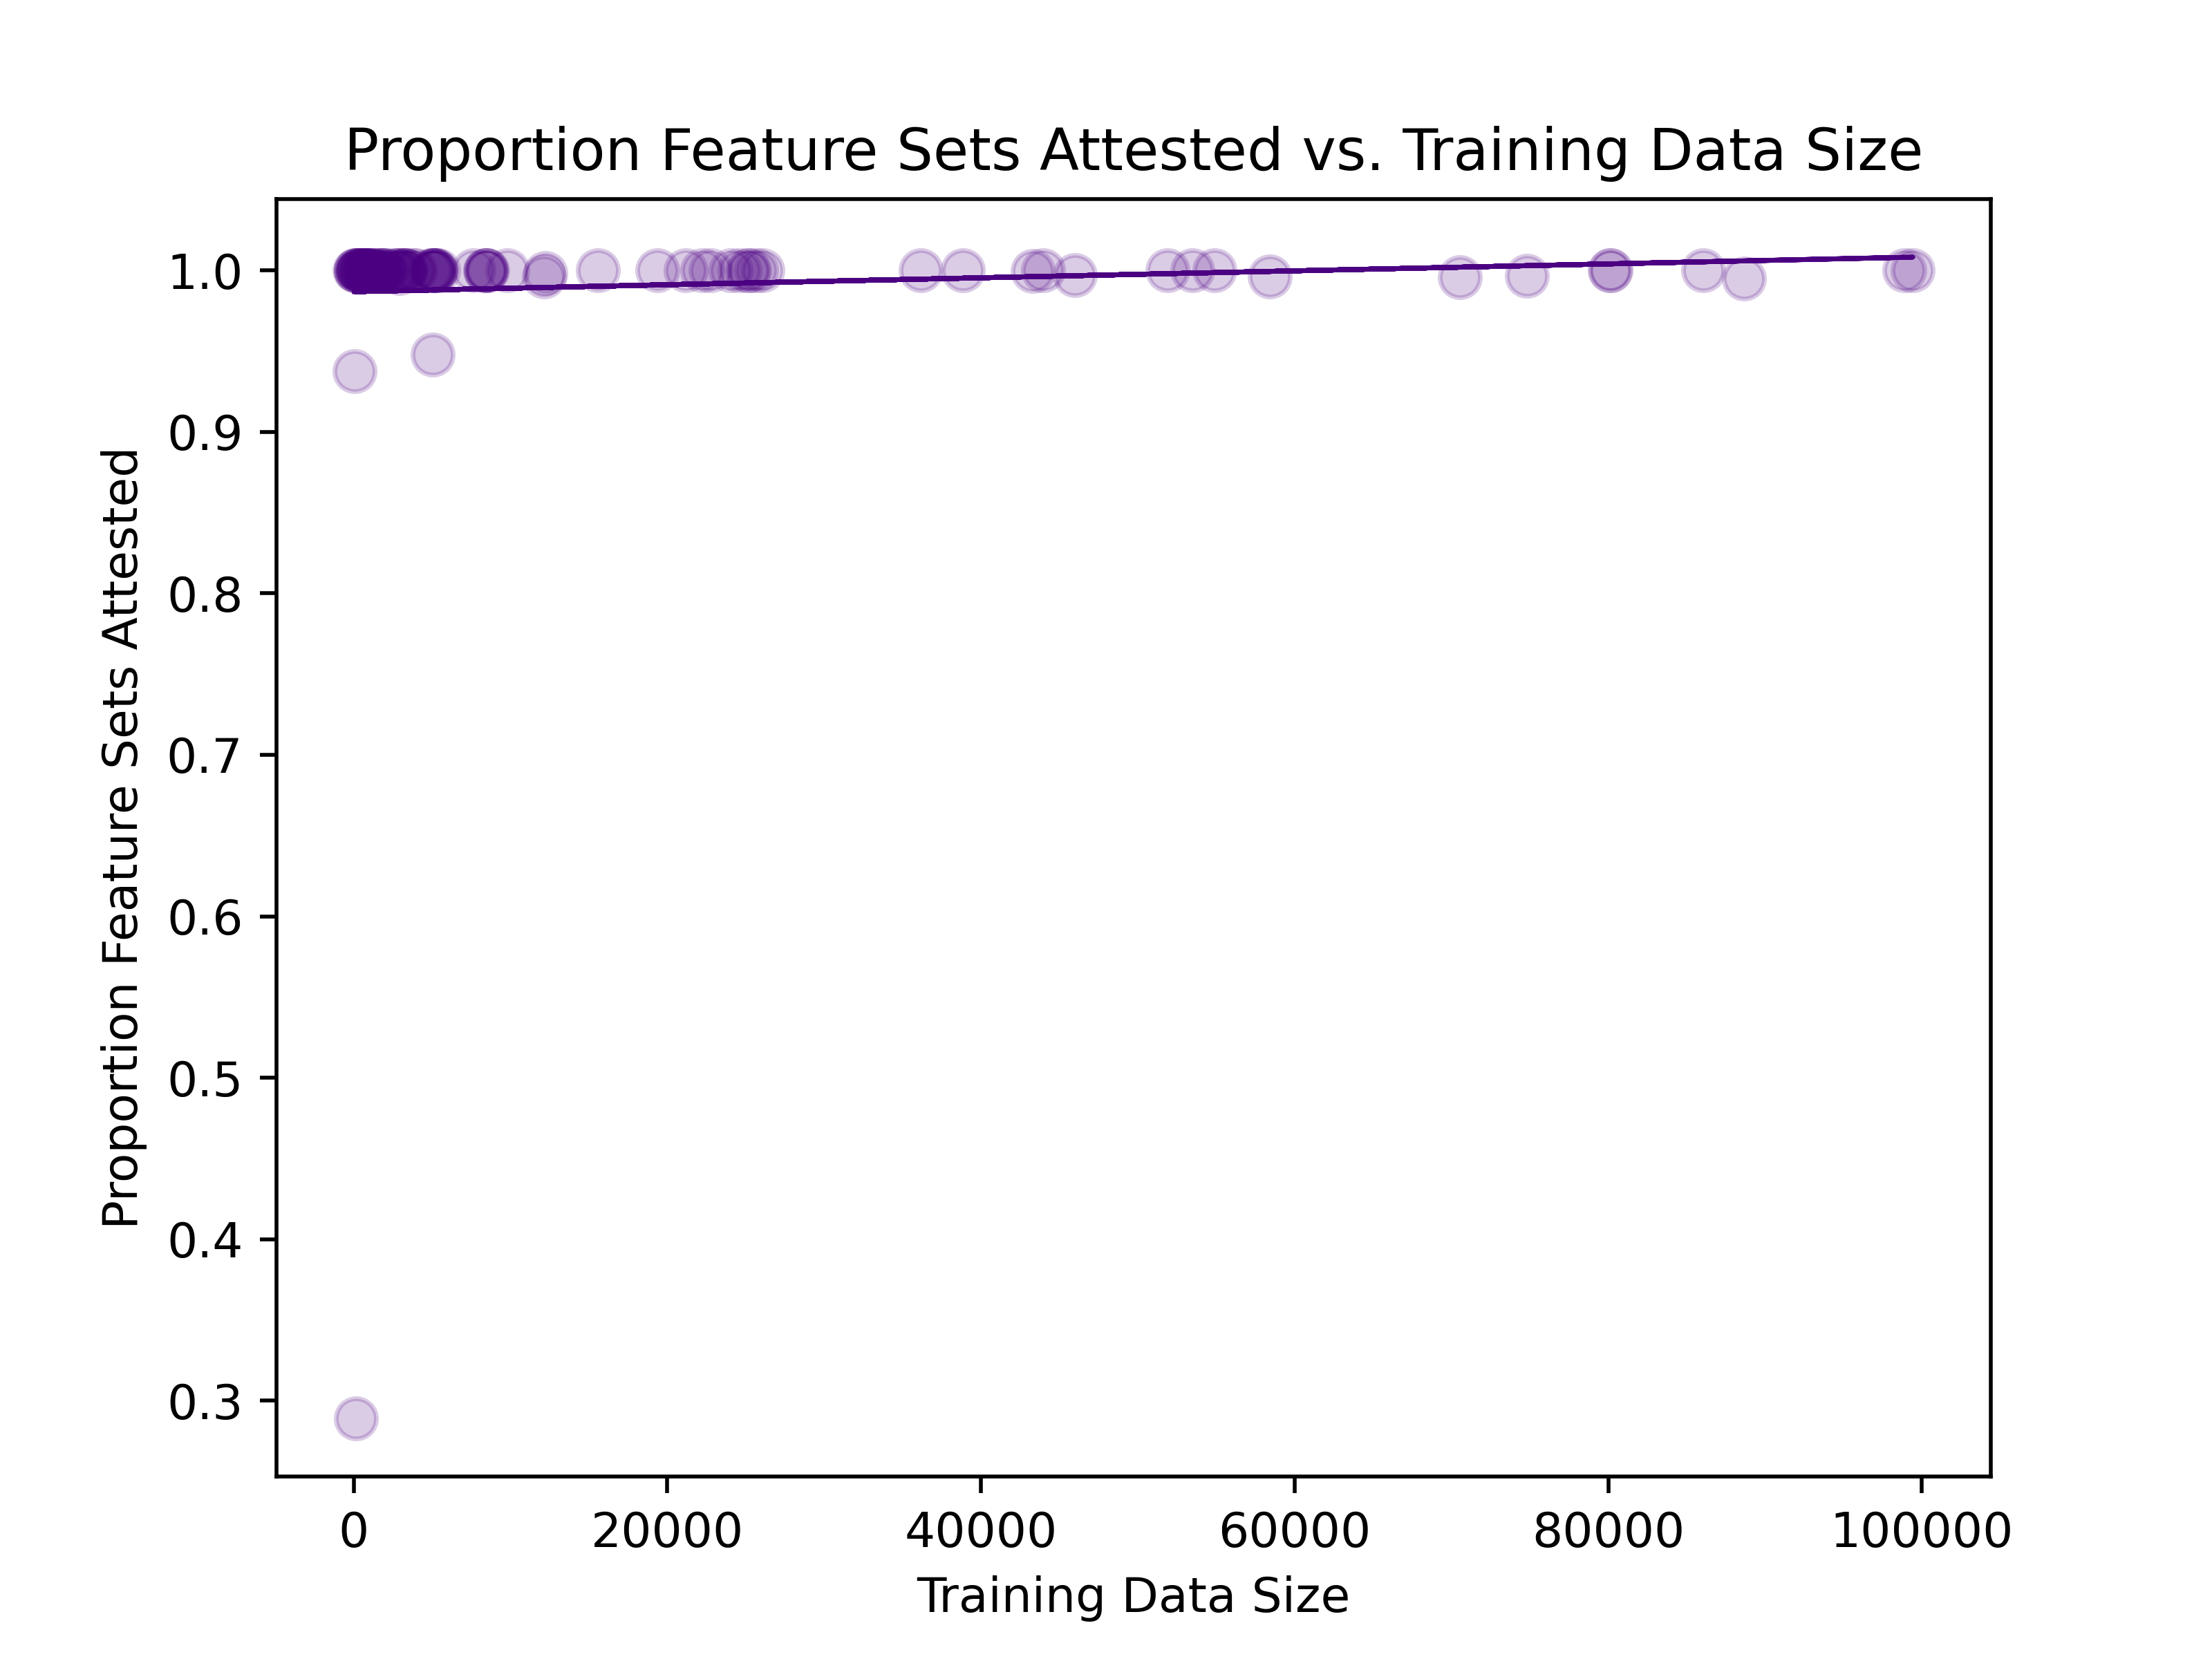
\includegraphics[width=\linewidth]{figs/feats_attested.png}
\caption{The proportion of feature sets appearing in test that have been seen in train+dev, as a function of training data size.}
\label{feats_attested}
\end{figure}

Under \citeauthor{goldman-etal-2022-un}'s lemma-based splitting, we would expect that feature overlap should always be 100\%. 
Since \textit{entire paradigms} are placed either in test or train, as long as there is another lemma of the same part of speech in the training data, then since the training lemma appears in its full paradigm, it should be the case that we have already seen all of the test features. 
For example, if \todo{add example}.
There are, of course, a few caveats to this point. 
Firstly, it assumes that every part of speech that appears in test will also appear in train. However, this assumption is entirely tenable given a moderate data sample, and \todo{check to see if it's the case that there's 100\% POS overlap}. 
Secondly, it assumes that the lemmas of the same POS in train don't have gaps -- for example, if \textit{stride} is the only verb we've seen in train, we likely won't have seen the past participle in train. 
However, it seems that this is also a tenable assumption given a moderate data sample. 

Indeed, when we examine the feature overlap in the data used by \citet{goldman-etal-2022-un} (Figure \ref{feats_attested}), we find that the feature overlap for most languages is 100\%. 
Indeed, there is little relationship between featureset overlap and training size (Pearson's $r = 0.068~(p=0.52)$, Spearman's $\rho = -0.254~(p=0.015)$, Kendall's $\tau_B = -0.207~(p = 0.014)$).
However, it is clearly not the case for all languages: the most dramatic outlier, Ludic, for example, has a feature overlap of just 0.303, meaning that less than a third of the feature sets appearing in the test data are attested in the train+dev. 
Preliminary examination of the Ludic data finds that this low overlap is due to just \textit{three} of the 26 total lemmas appearing in the test data. 
One of these lemmas, \textit{astuda}, appears with a whopping 131 feature sets in the testing data. 
We can ask whether it's reasonable to expect the model to be able to generate all 131 of these feature pairings by comparing the size of this test paradigm to comparable paradigms in train. 
In this case, \textit{astuda} is a verb, and the average size of a verbal paradigm in the Ludic training data is just 1.632 featuresets (stdev = 0.985). 
The largest verbal paradigm in the Ludic training data contains just 5 feature sets. 

It seems, then, that cases where \citeauthor{goldman-etal-2022-un}'s sampling strategy does not yield 100\% feature set overlap emerge as a result of data issues. 
\todo{A word about Ludic and the generation}
Though Ludic is by far the most glaring example, this pattern extends to other languages for which overlap is less than 100\%. 
To quantify this, we measure the difference in paradigm size between the \texttt{problematic lemmas} --- those appearing with at least one unattested featureset in test --- and the average paradigm size of words with the same part of speech in the training data.
We scale this value by the average paradigm size of words of the given part of speech in the training data so this number can be thought of as a \textit{proportional increase} in paradigm size.  
In other words, we measure: \todo{Just say this is measuring percent increase} 

\begin{footnotesize}
$$\frac{\texttt{avg. problematic lemma size - avg. train size}}{\texttt{avg. train size}}$$
\end{footnotesize}

For each part of speech for which there is at least one problematic lemma in the languages with overlap of under 100\%. 
Indeed, we find that the mean proportional difference is 4.825\% (stdev 8.948), with a large standard deviation stemming from a  number of large positive outliers. 
To give a point of comparison, we also measure the percent increase from the average training paradigm size to the \textit{maximum} test paradigm size across all POS for all languages for which there is 100\% overlap. 
Here, the percent increase is only 0.119\% (stdev 0.332); indeed, an unpaired T-test finds a significant difference between these two measures of increase ($t=5.801 (p=3.7*10^{-8})$).
The difference in these distributions is visualized in \todo{}

\begin{figure}
\centering
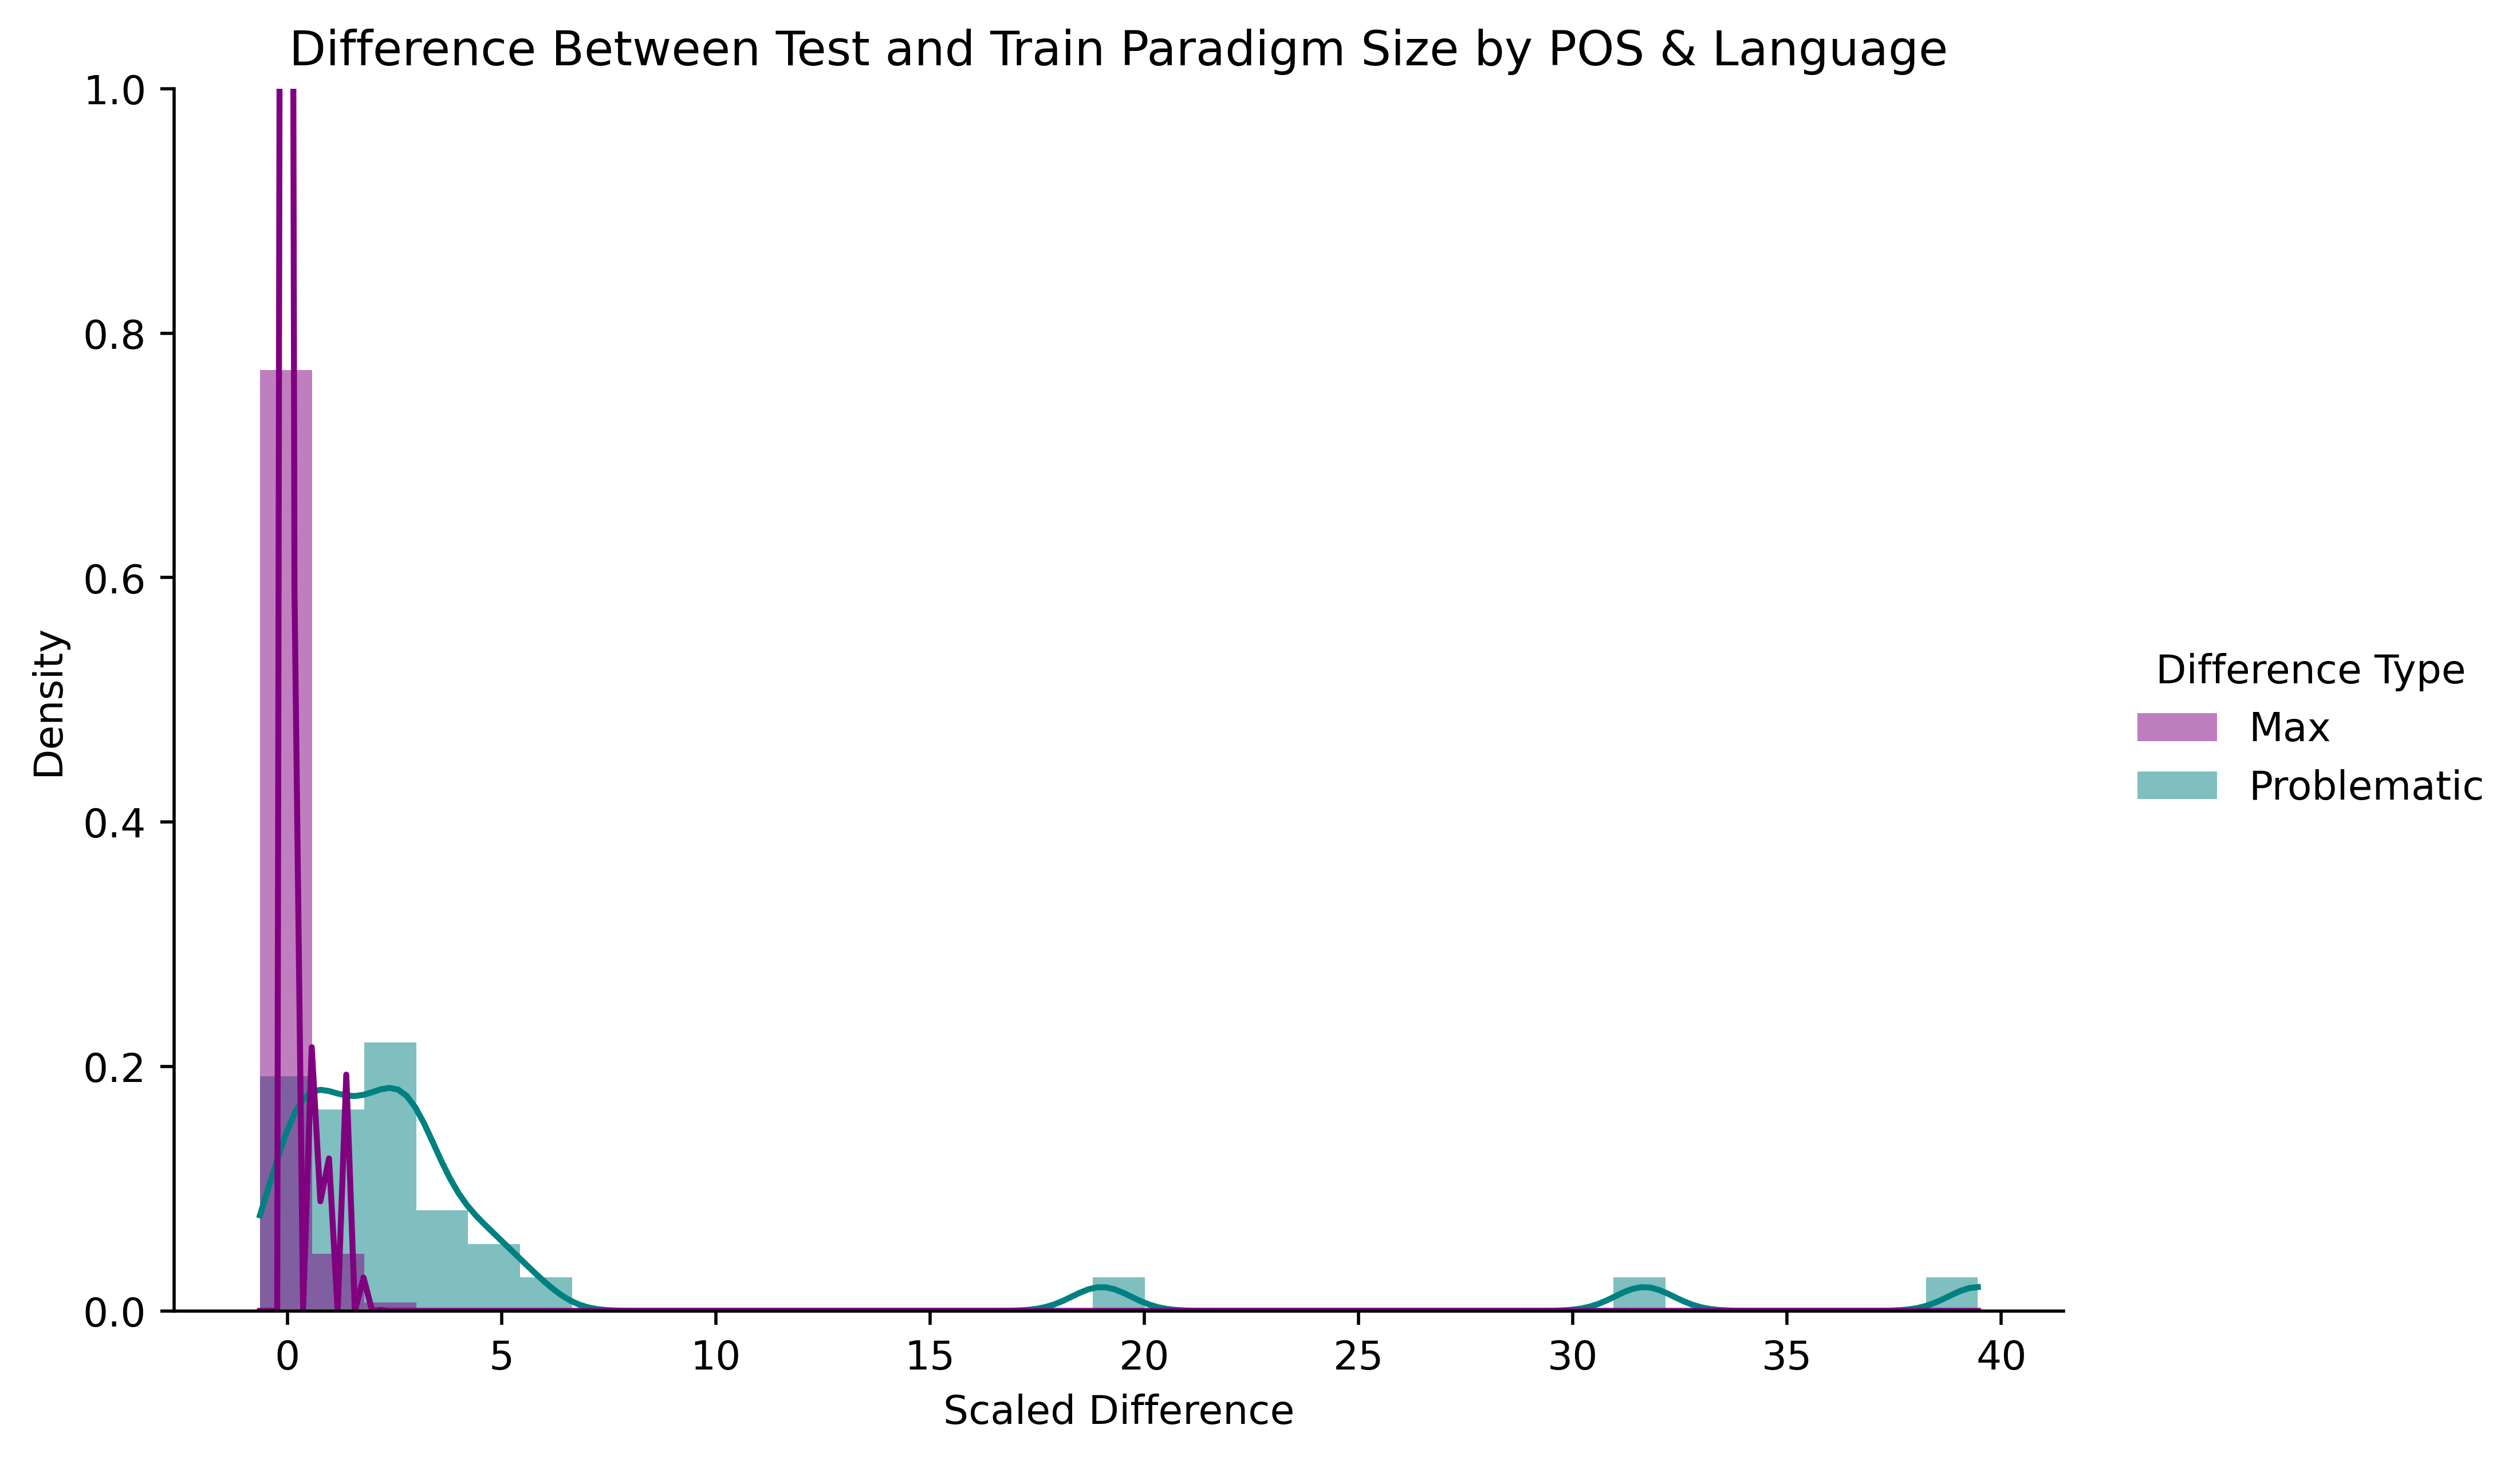
\includegraphics[width=\linewidth]{figs/percent_increase.png}
\caption{The proportion of feature sets appearing in test that have been seen in train+dev, as a function of training data size.}
\label{feats_attested}
\end{figure}

\newpage






% Bibliography entries for the entire Anthology, followed by custom entries
\bibliography{anthology,custom}
% Custom bibliography entries only
%\bibliography{custom}

%\appendix
%
%\section{Example Appendix}
%\label{sec:appendix}
%
%This is an appendix.

\end{document}
